\documentclass[conference]{IEEEtran}
\usepackage{cite}
\usepackage{amsmath,amssymb,amsfonts}
\usepackage{algorithmic}
\usepackage{graphicx}
\usepackage{textcomp}
\usepackage{xcolor}
\usepackage[all]{nowidow}
\usepackage[none]{hyphenat}

\newenvironment{Figure}
  {\par\medskip\noindent\minipage{\linewidth}}
  {\endminipage\par\medskip}

\def\BibTeX{{\rm B\kern-.05em{\sc i\kern-.025em b}\kern-.08em
    T\kern-.1667em\lower.7ex\hbox{E}\kern-.125emX}}
\begin{document}

\title{IoT based LPG Gas Utility system}

\author{
    \IEEEauthorblockN{
        Mitrajeet Golsangi\IEEEauthorrefmark{1},
        Divija Godse\IEEEauthorrefmark{2},
        Vivek Ghuge\IEEEauthorrefmark{3},\\
        Vishwajeet Haralkar\IEEEauthorrefmark{4},
        Adityaraj Honraopatil\IEEEauthorrefmark{5} and
        Dr. Vijay Gaikwad\IEEEauthorrefmark{6}
    }
    \IEEEauthorblockA{
        \textit{dept. of Computer Science} \\
        \textit{Vishwakarma Inststute of Technology}\\
        Pune, India\\
        Email : \IEEEauthorrefmark{1}mitrajeet.golsangi20@vit.edu,
        \IEEEauthorrefmark{2}divija.godse20@vit.edu,
        \IEEEauthorrefmark{3}vivek.ghuge20@vit.edu,\\
        \IEEEauthorrefmark{4}vishwajeet.haralkar20@vit.edu,
        \IEEEauthorrefmark{5}adityaraj.honraopatil20@vit.edu,
        \IEEEauthorrefmark{6}vijay.gaikwad@vit.edu,
    }
}


\maketitle

\begin{abstract}
    LPG is a powerful and efficient fuel that is primarily
    used in private cooking areas. LPG is highly combustible
    and can cause a fire even if it is far away from the
    source of the leak. The majority of fires are caused by
    a faulty rubber tube or when the regulator is not turned
    off. The proposed system is built around a microcontroller
    that includes gas sensors, GSM, a display, and a buzzer.
    The gas leak will be detected by the sensor, which will
    then send the information to the microcontroller. Based
    on that microcontroller makes a decision and displays a
    warning message. Another issue is the user not being
    able to tell the level of LP gas in the cylinder causing
    problems at the 11th hour. The proposed solution has
    brought a feasible solution to the same causing the
    users to monitor the Gas level from their mobile phones.
\end{abstract}

\begin{IEEEkeywords}
    LPG, IoT, LPG hazards, LPG monitoring , IoT embedded system
\end{IEEEkeywords}

\section{Introduction}
Our aim is to do a complete evaluation of the LPG
gas systems which have been rooted in nearly 30
crore people in India.\cite{[8]} It is a tedious process to
check the level of gas cylinder at home without any
special equipment and book the new one in anticipation.
We aim to improve the safety, usability and effectiveness
of the LPG gas cylinder.\\

LPG gas safety is a very important aspect of the
complete system. Gas leakage leads to various accidents
resulting in both financial loss as well as human
injuries.\cite{[6]} The risk of firing, explosion, suffocation
all are based on their physical properties such as
flammability, toxicity etc. According to the Ministry
of Petroleum and Natural Gas, Government of India
over 835 deaths have been recorded in 2018-19 in
India alone.\cite{[7]} Inspections by oil companies found that
many LPG consumers are unaware of safety checks of gas
cylinders. There is a need for a system to detect and
also prevent leakage of LPG.

\section{Literature Survey}
In these papers, the authors have mentioned the
use of an MQ-6 gas sensor, for the sole purpose
of leakage detection.\cite{[1]} The MQ-6 sensor senses LPG
leakage in any case and sends alert signals to the
microcontroller when it reaches a dangerous level.
Calculation: power of sensitivity\\[0.3em]
$P_s = V_c^2 \times \frac{R_s}{(R_s+R_L)^2}$\\[0.3em]
Resistance of sensor ($R_s$):\\[0.3em]
$R_s=\frac{V_c}{V\times R_L - 1}\times R_L$ \cite{[3]}\cite{[4]}\\
From the microcontroller, the alert signals are then
sent to the users via GSM.\cite{[2]} Thus the users would be
made aware of any kind of LPG leakage. Weight sensor
is used for the purpose of monitoring and detecting
the amount of gas present in the LPG cylinder.\cite{[3]}
Usually, the permissible net weight for LPG in the
domestic cylinder is 14kg. The weight of an empty
cylinder is approximately 15.3kg. The total gross
weight of the cylinder can be rounded off to
29.5kg. Thus when this figure changes the weight
sensor senses the smallest changes which are
further displayed on the LCD. When it reaches
0.5kg the system sends an alert to the user
device.\cite{[4]}

To address the above mentioned issues our project
uses the MQ-135 Gas sensor and alerts the user if the
regular gas composition of the surrounding atmosphere
changes. Our project would also use a 4.08mm force
sensor in combination with the Gas Sensor for
calculating the weight of the cylinder and notifying
the user if a certain threshold is crossed.
We intend to combine these two sensors and create a
system that would prevent gas leakage and also serve
as an alert sending device to prevent last minute
shortage.

Many solutions have been in the industry for years like
a solution created by students of KIIT \cite{[7]}.
The proposed solution aims to improve the safety,
usability and effectiveness of the LPG gas cylinder
usage. The advantages of the system are:
As the Weight sensor output is converted to digital
in the reference system there is a loss of accurate
data on actually how much level of gas is remaining
in the cylinder. The proposed systems avoids this
problem By using the Node MCU which has a built in
ESP8266 WiFi module the cost of the project has been
reduced By giving the user an application to monitor
their gas systems the accessibility and control over
the system have been increased significantly

\section{Methodology}

\begin{Figure}
    \centering
    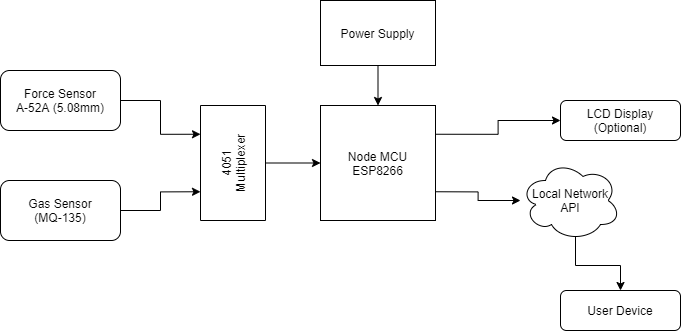
\includegraphics[width=\linewidth]{Images/BlockDiagram.png}
    \label{block}
    \figurename{Block Diagram}
\end{Figure}
The oversimplified block diagram (fig. \ref{block}) allows the users to
see the basic workflow of the project. The 4051
multiplexer toggles the analog input on the Node MCU
(pin A0) which is controlled by three pins D1, D2, D3
on Node MCU. The maximum amount of time is given for
the gas leakage detection whereas a finite amount of
time (not sure exactly how much yet) is given to the
Measurement of the level of gas in the cylinder. All
the statistics is sent to a host on the local network
and then is fetched from the user's application to give
him/her the most accurate data in real time.
\begin{Figure}
    \centering
    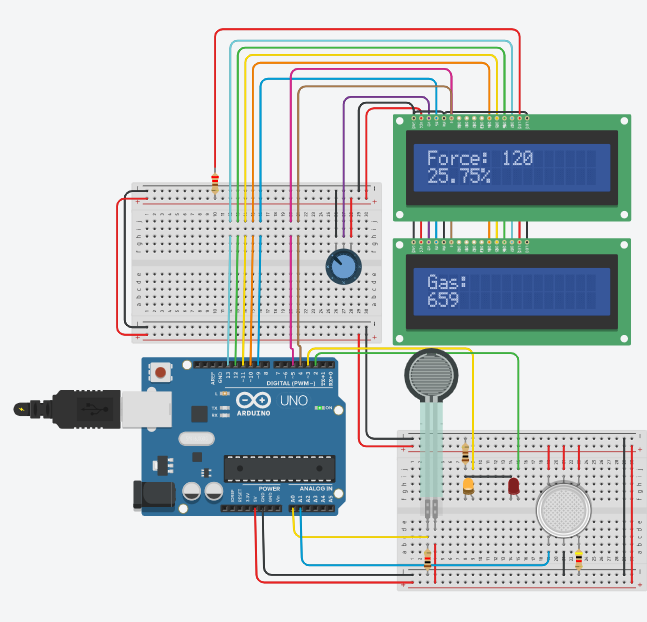
\includegraphics[width=\linewidth]{Images/Simulation.png}
    \label{sim}
    \figurename{Simulation}
\end{Figure}
figure \ref{sim} shows the simulation of the project that
has been performed on Autodesk TinkerCAD®. Here 2 LCD
monitors are used as wireless transmission cannot be
simulated. As seen the readings of the force and gas
Sensor are shown on the user device (LCD Display in
this case) and as the gas has crossed the soft
threshold of 470 PPM. The Yellow LED has been lit
up to warn the user of some abnormal Gas concentrations
in the surrounding atmosphere.

\subsection{Hardware}
\subsubsection{Part Required}
\begin{itemize}
    \item Node MCU 0.9 (ESP8266 Module)
    \item MQ-135 Gas Sensor
    \item A-52A 5.08mm Gas Sensor
    \item 4051N Multiplexer IC
    \item Resistors
    \item LED
    \item 15 pin female socket
\end{itemize}
\subsubsection{PCB Creation}
After the gathering of required components the team created a
schematic for the required circuit.
\begin{Figure}
    \centering
    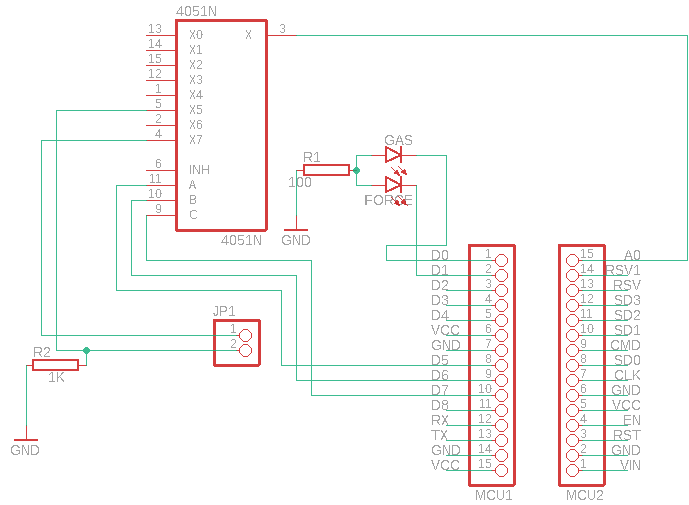
\includegraphics[width=\linewidth]{Images/Schematic.png}
    \label{schem}
    \figurename{Schematics}
\end{Figure}
After completion of the schematic and checking the connections the PCB board
layout was designed and finalized as shown below

\subsection{Software}
\subsubsection{Used Softwares}
\begin{itemize}
    \item VS Code IDE
    \item Platform IO IDE
    \item Eagle
\end{itemize}

\bibliographystyle{IEEEtran}
\bibliography{references.bib}

\end{document}
